\documentclass{beamer}

% {{{ beamer stuffs
\setbeamertemplate{footline}[frame number]
\beamertemplatenavigationsymbolsempty%
\logo{
\includegraphics[height=4mm]{fig/LogoEnseeiht.png}}
\usetheme{Montpellier}
\usecolortheme{dolphin}
% }}}

\usepackage{fontspec}
\usepackage{hyperref}
\usepackage{pdflscape}

\title{CRAPS Kernel}
\subtitle{Final presentation}
\author{
       Maxime Arthaud
  \and Korantin Auguste
  \and Martin Carton
  \and Étienne Lebrun
}
\titlegraphic{
\includegraphics[width=0.5\textwidth]{fig/LogoEnseeiht.png}}
\date{March 13, 2015}

\begin{document}
  \begin{frame}[plain]
    \titlepage%
  \end{frame}

  \begin{frame}[plain]
    \tableofcontents
  \end{frame}

  \section{The project}
    \begin{frame}{Presentation}
      \begin{itemize}
        \item Implement a basic operating system on CRAPS
          \begin{itemize}
            \item CRAPS: processor architecture developed by Jean-Christophe
              Buisson for first year students
          \end{itemize}
        \item Goal: make a operating system course
          \begin{itemize}
            \item based on what student know
            \item adding a continuity in courses
          \end{itemize}
      \end{itemize}
    \end{frame}

    \begin{frame}[plain]
      \begin{figure}
        \centering
        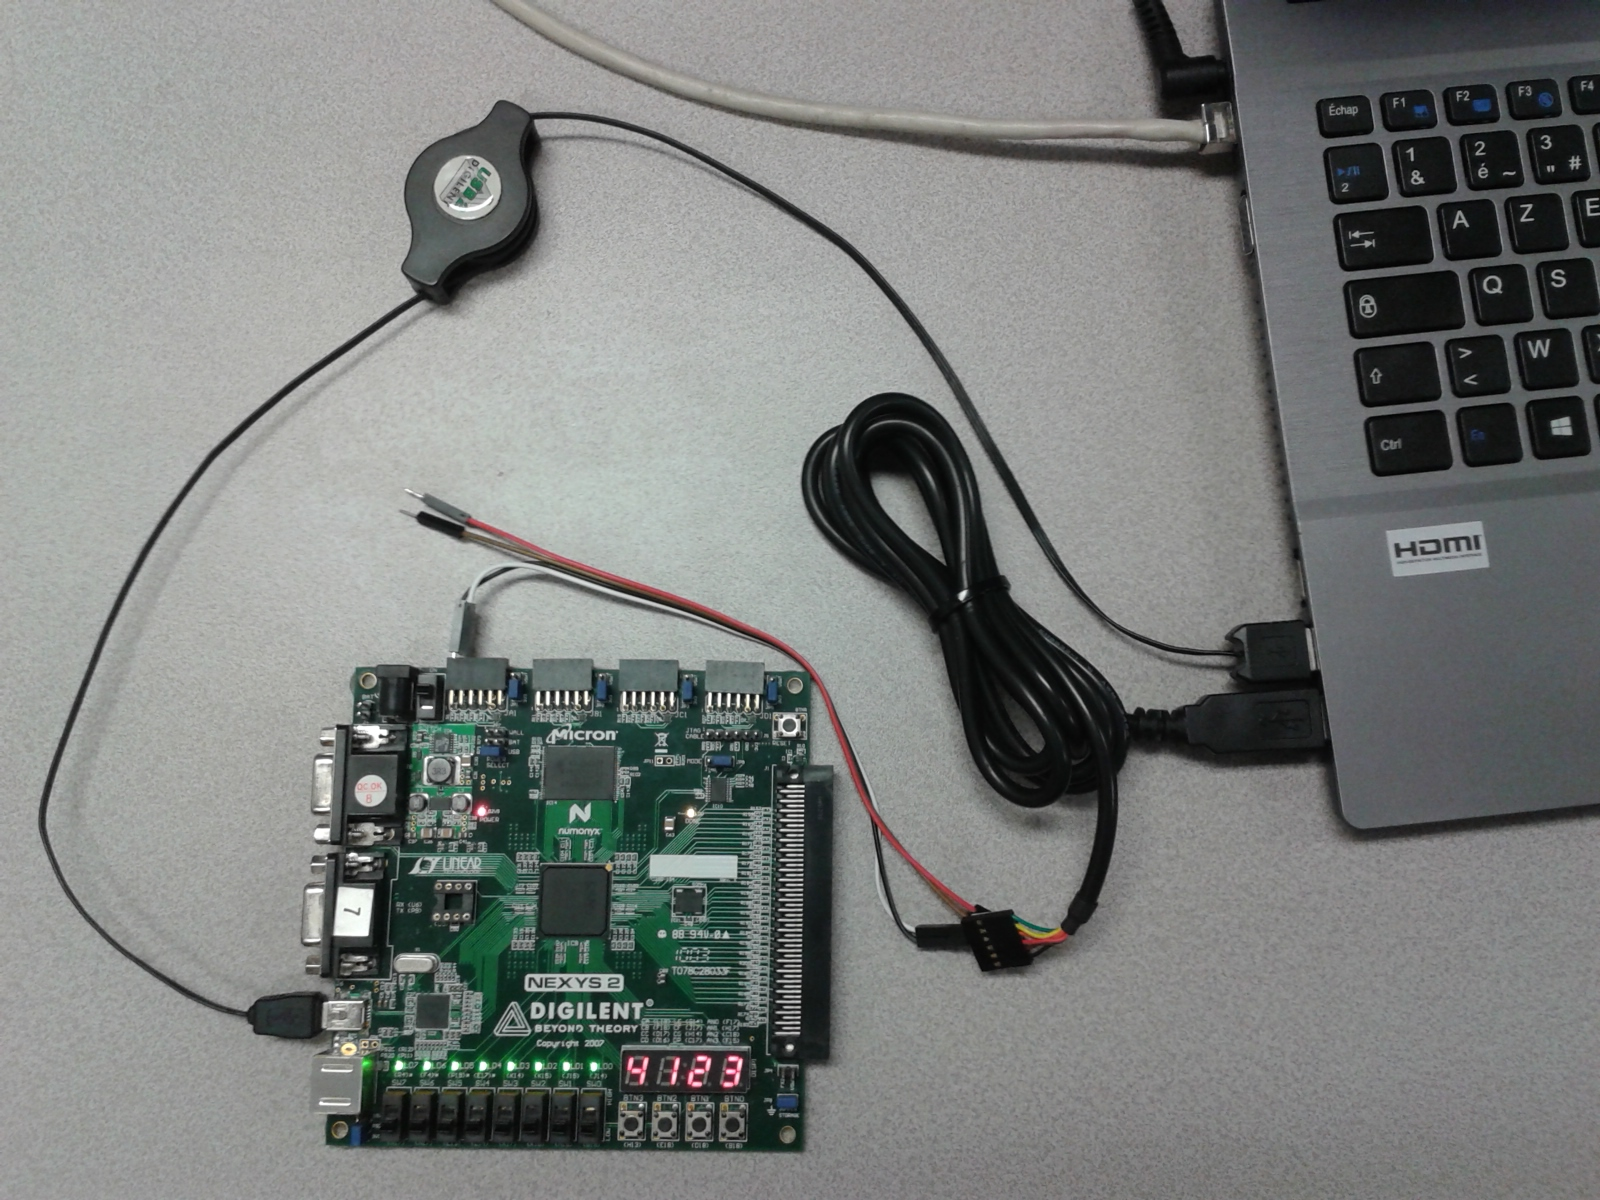
\includegraphics[width=\textwidth, keepaspectratio]{fig/Nexys2.jpg}
        \caption{A Nexys2 board}
      \end{figure}
    \end{frame}

    \begin{frame}{Goal}
      It should show students how a basic operating system works:
        \begin{itemize}
          \item scheduling
          \item interrupts
          \item communications
          \item memory management
        \end{itemize}
    \end{frame}

  \section{Project management}
    \subsection{Team}
      \begin{frame}{Team organization}
        \begin{itemize}
          \item Korantin Auguste as \textit{developer}
          \item Maxime Arthaud as \textit{tester}
          \item Martin Carton as \textit{project leader}
          \item Étienne Lebrun as \textit{quality manager}
        \end{itemize}
      \end{frame}

    \subsection{Project organization}
      \begin{frame}{Risks management}
        We were able to identify real risks, and mitigate them:
        \begin{itemize}
          \item Damaged FPGA
          \item Unable to integrate more RAM
          \item Serial too slow
        \end{itemize}
      \end{frame}

      \begin{frame}{Specifications}
        \begin{itemize}
          \item First week of the project
          \item We identified three main tasks:
            \begin{itemize}
              \item The compiler
              \item The modifications to the processor
              \item The kernel
            \end{itemize}
          \end{itemize}
      \end{frame}

      \begin{frame}{Calendar}
      \end{frame}

      \begin{frame}[plain]
        \begin{figure}
          \includegraphics[height=\textheight, width=\textwidth, keepaspectratio]
                          {build/Gantt.pdf}
        \end{figure}
      \end{frame}

      \begin{frame}{Team management}
        Quite free, working on what we like.

        \begin{center}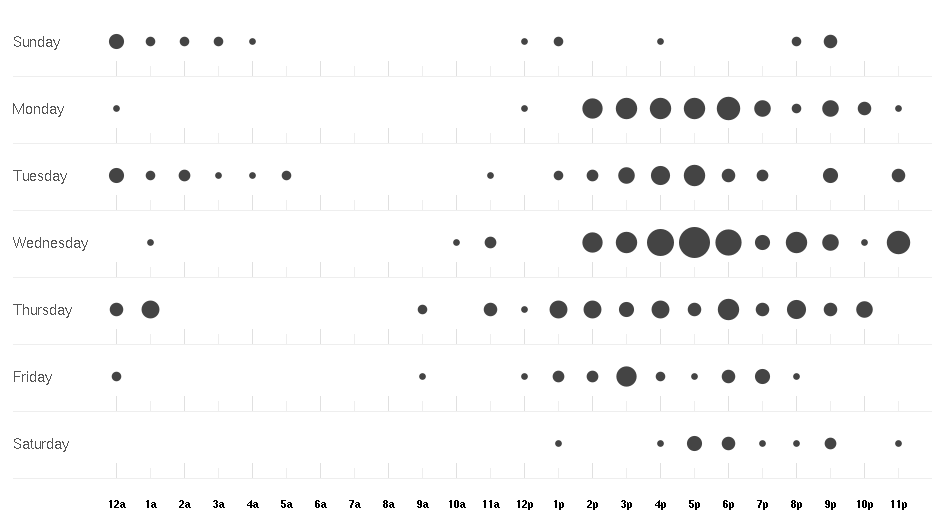
\includegraphics[scale=0.35]{fig/punchcard.png}\end{center}
      \end{frame}

      \begin{frame}{Deliverables}
        \begin{itemize}
          \item Documentation and manual for students and teachers
            \begin{itemize}
              \item What we changed
              \item How to use our tools
              \item The syntax of our language
              \item \dots
            \end{itemize}
          \item Kernel, compiler, new processor
          \item Reports, abstract
        \end{itemize}
      \end{frame}

  \section{Processor Changes}
    \begin{landscape}
        \begin{frame}[plain]
            \includegraphics[scale=0.22]
                            {build/micromachine_updated_fromsvg.pdf}

        \end{frame}
    \end{landscape}

  \section{Implementation}
    \begin{frame}{Compiler}
      \begin{itemize}
        \item Based on the compiler project from the second-year classes.
        \item Language: a (quite large!) subset of C.
        \item Various optimizations.
      \end{itemize}
    \end{frame}

    \begin{frame}{Interrupts}
      \begin{itemize}
        \item Processor modifications.
        \item Priority support.
        \item Interrupt table.
      \end{itemize}
    \end{frame}

    \begin{frame}{Scheduler}
      Needed to make "context switch": change the current process.

      \begin{center}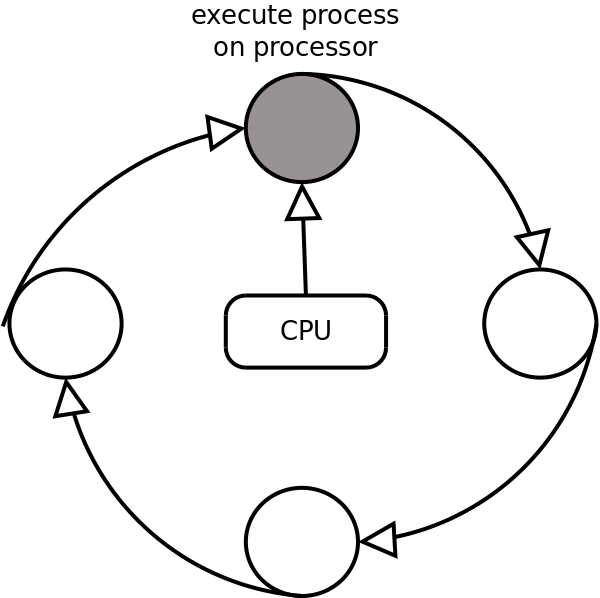
\includegraphics[scale=0.2]{fig/rr.png}\end{center}

      Have to save the current state of the processor, restore the state for the other process, and continue.
    \end{frame}

    \begin{frame}{Scheduler}
      \begin{itemize}
        \item New interrupt based on the PWM, that will trigger a context switch.
        \item Context switch:
        \begin{enumerate}
           \item Save the registers on the current stack
           \item Change the current stack to the one of the next process
           \item Restore the registers
           \item Return from interrupt (will jump to the address of the instruction stored on the stack of the new process)
        \end{enumerate}
      \end{itemize}
    \end{frame}

    \begin{frame}{Serial Port}
      To communicate with the computer we used a serial port.

      \pause
      We had to modify the processor:
      \begin{itemize}
        \item Add a new built-in module in SHDL
        \item Add a new interrupt in the processor
        \item Map the module to memory
      \end{itemize}

      \pause
      We had some problems:
      \begin{itemize}
        \item the module can cause the synthesis to fail (too complex?)
        \item the communication is slow, we can lose data
      \end{itemize}
    \end{frame}

    \begin{frame}{Memory Management}
      \begin{itemize}
        \item We need to be able to dynamically allocate memory.
        \item In modern computers: virtual memory (segmentation and pagination). Too complicated.
        \item We just need three functions: malloc, free, realloc.
        \item How to free all the memory of a process ?
      \end{itemize}
    \end{frame}
    
    \begin{frame}{Memory Management}
      \begin{itemize}
        \item Stored in blocks, with a header indicating the size and the PID of the owner.
        \item All blocks have a size that is a power of two.
        \item We never split/merge/delete blocks, we just reuse them if freed.
        \item We can free all the blocks for a given process.
      \end{itemize}
    \end{frame}

    \begin{frame}[plain]
      \begin{figure}
        \begin{minipage}[c]{0.5\textwidth}
          \caption{Memory layout}
        \end{minipage}\hfill
        \begin{minipage}[c]{0.5\textwidth}
          \includegraphics[height=\textheight]{build/memory_layout_fromsvg.pdf}
        \end{minipage}
      \end{figure}
    \end{frame}

    \subsection{Dynamic loading}
      \begin{frame}
        \begin{itemize}
          \item Not very hard to do\dots
          \item \dots but we had to make the code position-independent.
        \end{itemize}
      \end{frame}

  \section{Final result}
    \begin{frame}{Various processes}
      \begin{itemize}
        \item The shell (most important)
        \item Counter
        \item Leds
        \item \dots and dynamic loading!
      \end{itemize}
    \end{frame}

    \begin{frame}{Demo}
      \begin{itemize}
        \item Compiler
        \item Debugger
        \item Serial console
        \item Process management
      \end{itemize}
    \end{frame}

  \section{Use/Improvements}
    \begin{frame}{Pedagogic use}
        Use in classes? Pedagogic interest.
    \end{frame}

  \section{Questions}
    \begin{frame}
      Any questions?
    \end{frame}
\end{document}
